\documentclass[ ]{article}

\usepackage[ ]{graphicx}
\usepackage[ ]{amsmath}

\title{Revisão P2 de Probabilidade e Estatística \\ Leandro Bordin}
\author{Erickson G. Müller}
\date{19 de Junho de 2024}

\begin{document}

\maketitle
\section{Conteúdo}
\begin{enumerate}
	\item Estimação de Parâmetros
\end{enumerate}
\pagebreak

\section{Teoria da Estimação para uma Amostra}
	Existem dois tipos de dados para representar a amostra: Estimativa Pontual e Estimativa Intervalar. Como a variabilidade amostral pode resultar estimativas diferentes conforme as amostras selecionadas, agrega-se uma estimativa intervalar para acompanhar a estimativa pontual.

\subsection{Teorema do Limite Central}	
	A variabilidade amostral se	 comporta como uma distribuição normal para amostras maiores ou iguais a 30.

\subsection{Fórmulas da Estimativa}
	\begin{equation*}
		Estimativa Pontual: ux = \overline{x}
	\end{equation*}
	\begin{equation*}
		Estimativa Intervalar: ux = \overline{x} +- z.\dfrac{desvio padrao}{\sqrt[]{n}}
	\end{equation*}	
\subsection{Fórmulas da Proporção}
	\begin{equation*}
		Estimativa Pontual da Proporcao: p = \overline{p} = \dfrac{x}{n}
	\end{equation*}
	\begin{equation*}
		Estimativa Intervalar da Proporcao: p = \overline{p} \pm \sqrt[]{\dfrac{\overline{p}.(1-\overline{p})}{n}}
	\end{equation*}
\section{Teste de Hipóteses}
	Os testes de hipóteses, ou testes de significância e a estimação são os dois ramos principais da inferência estatística. O objetivo do teste de hipótese é decidir se determinada afirmação sobre um parâmetro populacional é verdadeira.
\subsection{Nível de Significância}
	 Dá a probabilidade de rejeitar a hipótese nula\\
	 
	 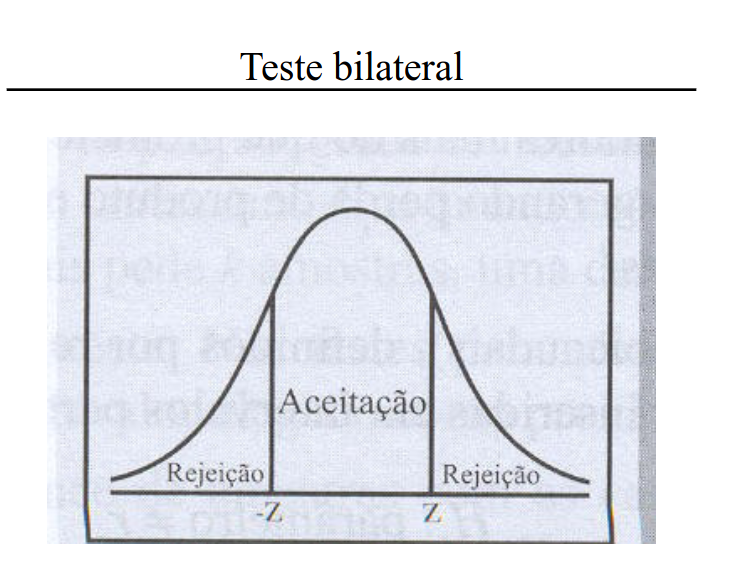
\includegraphics[scale=.3]{Images/H1 diff.png}
	 $$H_0 = // H_1 !=$$
	  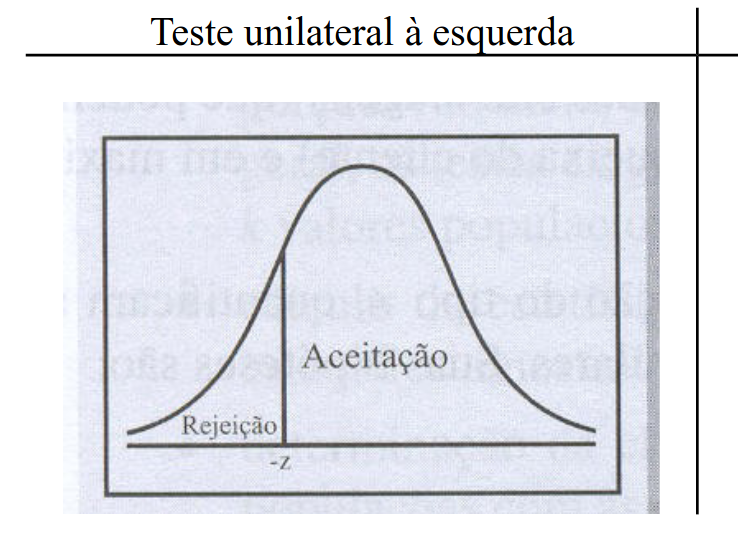
\includegraphics[scale=.3]{Images/H1 smaller.png}
	  $$H_0>= // H_1 <$$
	   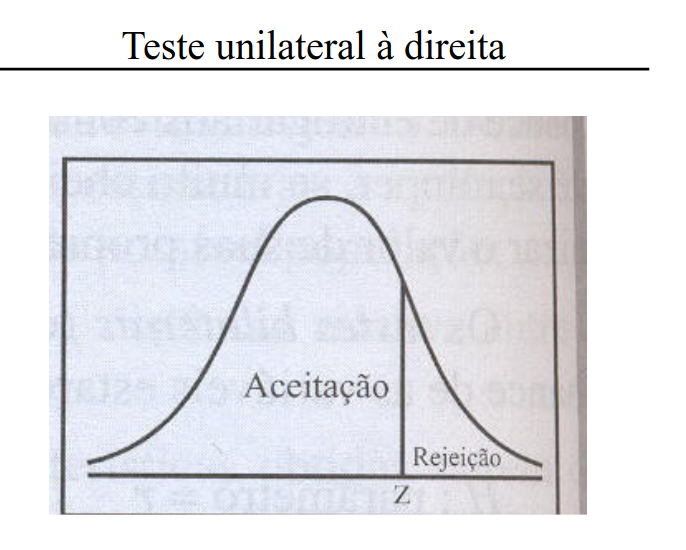
\includegraphics[scale=.3]{Images/H1 bigger.png}
	   $$H_0<= // H_1 >$$
\subsection{Etapas de um teste de hipótese}
	\begin{enumerate}
		\item Definir as hipóteses de teste: nula ($H_0$) e alternativa ($H_1$)
		\item Fixar um nível de significância $\alpha$
		\item Calcular o valor de estatística de teste:
		$$z_{teste}=\dfrac{parametro.da.amostra - parametro.alegado}{desvio.padrao.da.distribuicao.amostral}$$
		\item Estabelecer o valor crítico ou valores críticos da estatística de teste
		\item Comparar o valor da estatística de teste  com o valor crítico e tomar decisão: se o valor estiver na região de aceitação, aceita-se o $H_0$. Caso estiver na região de rejeição, rejeita-se o $H_0$ e se aceita o $H_1$.
	\end{enumerate}
\end{document}

